\documentclass[]{article}
\usepackage{lmodern}
\usepackage{amssymb,amsmath}
\usepackage{ifxetex,ifluatex}
\usepackage{fixltx2e} % provides \textsubscript
\ifnum 0\ifxetex 1\fi\ifluatex 1\fi=0 % if pdftex
  \usepackage[T1]{fontenc}
  \usepackage[utf8]{inputenc}
\else % if luatex or xelatex
  \ifxetex
    \usepackage{mathspec}
  \else
    \usepackage{fontspec}
  \fi
  \defaultfontfeatures{Ligatures=TeX,Scale=MatchLowercase}
\fi
% use upquote if available, for straight quotes in verbatim environments
\IfFileExists{upquote.sty}{\usepackage{upquote}}{}
% use microtype if available
\IfFileExists{microtype.sty}{%
\usepackage{microtype}
\UseMicrotypeSet[protrusion]{basicmath} % disable protrusion for tt fonts
}{}
\usepackage[margin=1in]{geometry}
\usepackage{hyperref}
\hypersetup{unicode=true,
            pdftitle={Tidy the data to the correct format},
            pdfauthor={Jeff Wesner},
            pdfborder={0 0 0},
            breaklinks=true}
\urlstyle{same}  % don't use monospace font for urls
\usepackage{color}
\usepackage{fancyvrb}
\newcommand{\VerbBar}{|}
\newcommand{\VERB}{\Verb[commandchars=\\\{\}]}
\DefineVerbatimEnvironment{Highlighting}{Verbatim}{commandchars=\\\{\}}
% Add ',fontsize=\small' for more characters per line
\usepackage{framed}
\definecolor{shadecolor}{RGB}{248,248,248}
\newenvironment{Shaded}{\begin{snugshade}}{\end{snugshade}}
\newcommand{\KeywordTok}[1]{\textcolor[rgb]{0.13,0.29,0.53}{\textbf{#1}}}
\newcommand{\DataTypeTok}[1]{\textcolor[rgb]{0.13,0.29,0.53}{#1}}
\newcommand{\DecValTok}[1]{\textcolor[rgb]{0.00,0.00,0.81}{#1}}
\newcommand{\BaseNTok}[1]{\textcolor[rgb]{0.00,0.00,0.81}{#1}}
\newcommand{\FloatTok}[1]{\textcolor[rgb]{0.00,0.00,0.81}{#1}}
\newcommand{\ConstantTok}[1]{\textcolor[rgb]{0.00,0.00,0.00}{#1}}
\newcommand{\CharTok}[1]{\textcolor[rgb]{0.31,0.60,0.02}{#1}}
\newcommand{\SpecialCharTok}[1]{\textcolor[rgb]{0.00,0.00,0.00}{#1}}
\newcommand{\StringTok}[1]{\textcolor[rgb]{0.31,0.60,0.02}{#1}}
\newcommand{\VerbatimStringTok}[1]{\textcolor[rgb]{0.31,0.60,0.02}{#1}}
\newcommand{\SpecialStringTok}[1]{\textcolor[rgb]{0.31,0.60,0.02}{#1}}
\newcommand{\ImportTok}[1]{#1}
\newcommand{\CommentTok}[1]{\textcolor[rgb]{0.56,0.35,0.01}{\textit{#1}}}
\newcommand{\DocumentationTok}[1]{\textcolor[rgb]{0.56,0.35,0.01}{\textbf{\textit{#1}}}}
\newcommand{\AnnotationTok}[1]{\textcolor[rgb]{0.56,0.35,0.01}{\textbf{\textit{#1}}}}
\newcommand{\CommentVarTok}[1]{\textcolor[rgb]{0.56,0.35,0.01}{\textbf{\textit{#1}}}}
\newcommand{\OtherTok}[1]{\textcolor[rgb]{0.56,0.35,0.01}{#1}}
\newcommand{\FunctionTok}[1]{\textcolor[rgb]{0.00,0.00,0.00}{#1}}
\newcommand{\VariableTok}[1]{\textcolor[rgb]{0.00,0.00,0.00}{#1}}
\newcommand{\ControlFlowTok}[1]{\textcolor[rgb]{0.13,0.29,0.53}{\textbf{#1}}}
\newcommand{\OperatorTok}[1]{\textcolor[rgb]{0.81,0.36,0.00}{\textbf{#1}}}
\newcommand{\BuiltInTok}[1]{#1}
\newcommand{\ExtensionTok}[1]{#1}
\newcommand{\PreprocessorTok}[1]{\textcolor[rgb]{0.56,0.35,0.01}{\textit{#1}}}
\newcommand{\AttributeTok}[1]{\textcolor[rgb]{0.77,0.63,0.00}{#1}}
\newcommand{\RegionMarkerTok}[1]{#1}
\newcommand{\InformationTok}[1]{\textcolor[rgb]{0.56,0.35,0.01}{\textbf{\textit{#1}}}}
\newcommand{\WarningTok}[1]{\textcolor[rgb]{0.56,0.35,0.01}{\textbf{\textit{#1}}}}
\newcommand{\AlertTok}[1]{\textcolor[rgb]{0.94,0.16,0.16}{#1}}
\newcommand{\ErrorTok}[1]{\textcolor[rgb]{0.64,0.00,0.00}{\textbf{#1}}}
\newcommand{\NormalTok}[1]{#1}
\usepackage{graphicx,grffile}
\makeatletter
\def\maxwidth{\ifdim\Gin@nat@width>\linewidth\linewidth\else\Gin@nat@width\fi}
\def\maxheight{\ifdim\Gin@nat@height>\textheight\textheight\else\Gin@nat@height\fi}
\makeatother
% Scale images if necessary, so that they will not overflow the page
% margins by default, and it is still possible to overwrite the defaults
% using explicit options in \includegraphics[width, height, ...]{}
\setkeys{Gin}{width=\maxwidth,height=\maxheight,keepaspectratio}
\IfFileExists{parskip.sty}{%
\usepackage{parskip}
}{% else
\setlength{\parindent}{0pt}
\setlength{\parskip}{6pt plus 2pt minus 1pt}
}
\setlength{\emergencystretch}{3em}  % prevent overfull lines
\providecommand{\tightlist}{%
  \setlength{\itemsep}{0pt}\setlength{\parskip}{0pt}}
\setcounter{secnumdepth}{0}
% Redefines (sub)paragraphs to behave more like sections
\ifx\paragraph\undefined\else
\let\oldparagraph\paragraph
\renewcommand{\paragraph}[1]{\oldparagraph{#1}\mbox{}}
\fi
\ifx\subparagraph\undefined\else
\let\oldsubparagraph\subparagraph
\renewcommand{\subparagraph}[1]{\oldsubparagraph{#1}\mbox{}}
\fi

%%% Use protect on footnotes to avoid problems with footnotes in titles
\let\rmarkdownfootnote\footnote%
\def\footnote{\protect\rmarkdownfootnote}

%%% Change title format to be more compact
\usepackage{titling}

% Create subtitle command for use in maketitle
\providecommand{\subtitle}[1]{
  \posttitle{
    \begin{center}\large#1\end{center}
    }
}

\setlength{\droptitle}{-2em}

  \title{Tidy the data to the correct format}
    \pretitle{\vspace{\droptitle}\centering\huge}
  \posttitle{\par}
    \author{Jeff Wesner}
    \preauthor{\centering\large\emph}
  \postauthor{\par}
      \predate{\centering\large\emph}
  \postdate{\par}
    \date{September 20, 2019}


\begin{document}
\maketitle

\begin{figure}
\centering
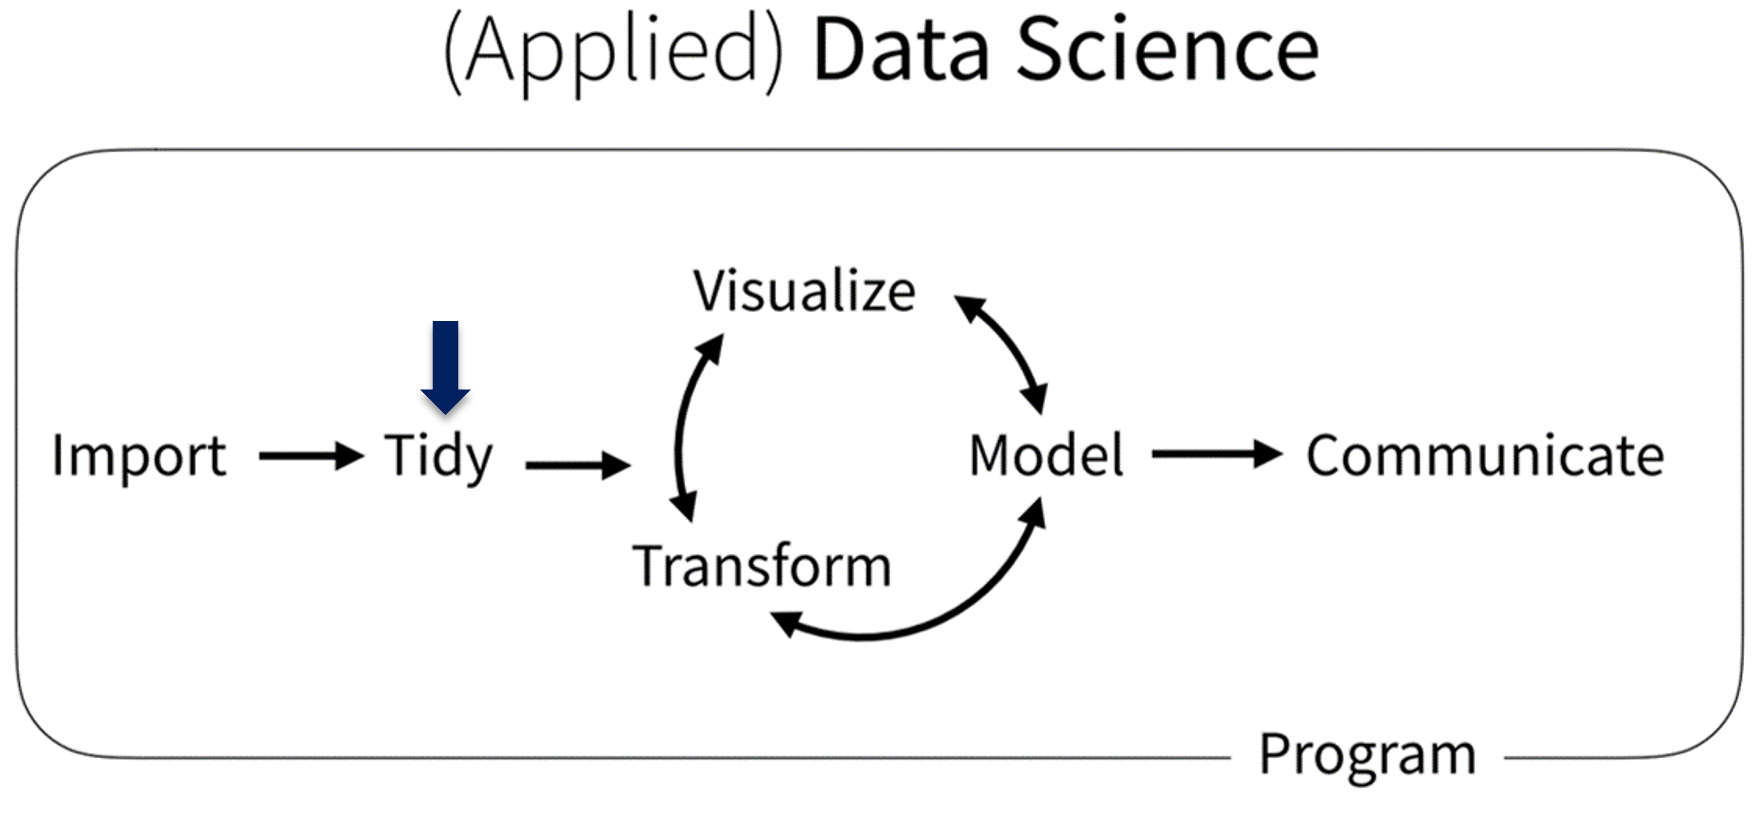
\includegraphics{data_workflow_tidy.png}
\caption{}
\end{figure}

\section{4) Tidy the data}\label{tidy-the-data}

Most datasets are formatted for humans to read. But computers want a
different format. The next steps will turn your dataset into a format
that your computer can read. We refer to it as ``tidy data''. You can
read more about it
\href{http://www.cs.umd.edu/class/fall2018/cmsc641/files/tidy_data.pdf}{here}
(but you don't have to). First we need to install some packages that
will make this process easy.

\subsubsection{Open a script}\label{open-a-script}

\emph{File -\textgreater{} New File -\textgreater{} R Script}

You should see a blank file with a flashing prompt. Script's are your
friend. It's where you tell the computer what to do. For example, you
might want to give your dataset a shorter name, since you'll have to
type it over and over again. Paste the code below in your script and
click \emph{Run}.

\begin{Shaded}
\begin{Highlighting}[]
\NormalTok{total_fertility <-}\StringTok{ }\NormalTok{children_per_woman_total_fertility}
\end{Highlighting}
\end{Shaded}

In words, this says ``create a new dataset called total\_fertility from
the other dataset called children\_per\_woman\_total\_fertility''. The
arrow is made with two symbols, a \emph{lesser than} \textless{} and a
\emph{minus} -, which gives \textless{}-.

If it worked, you should see two files in the upper right panel like
this: 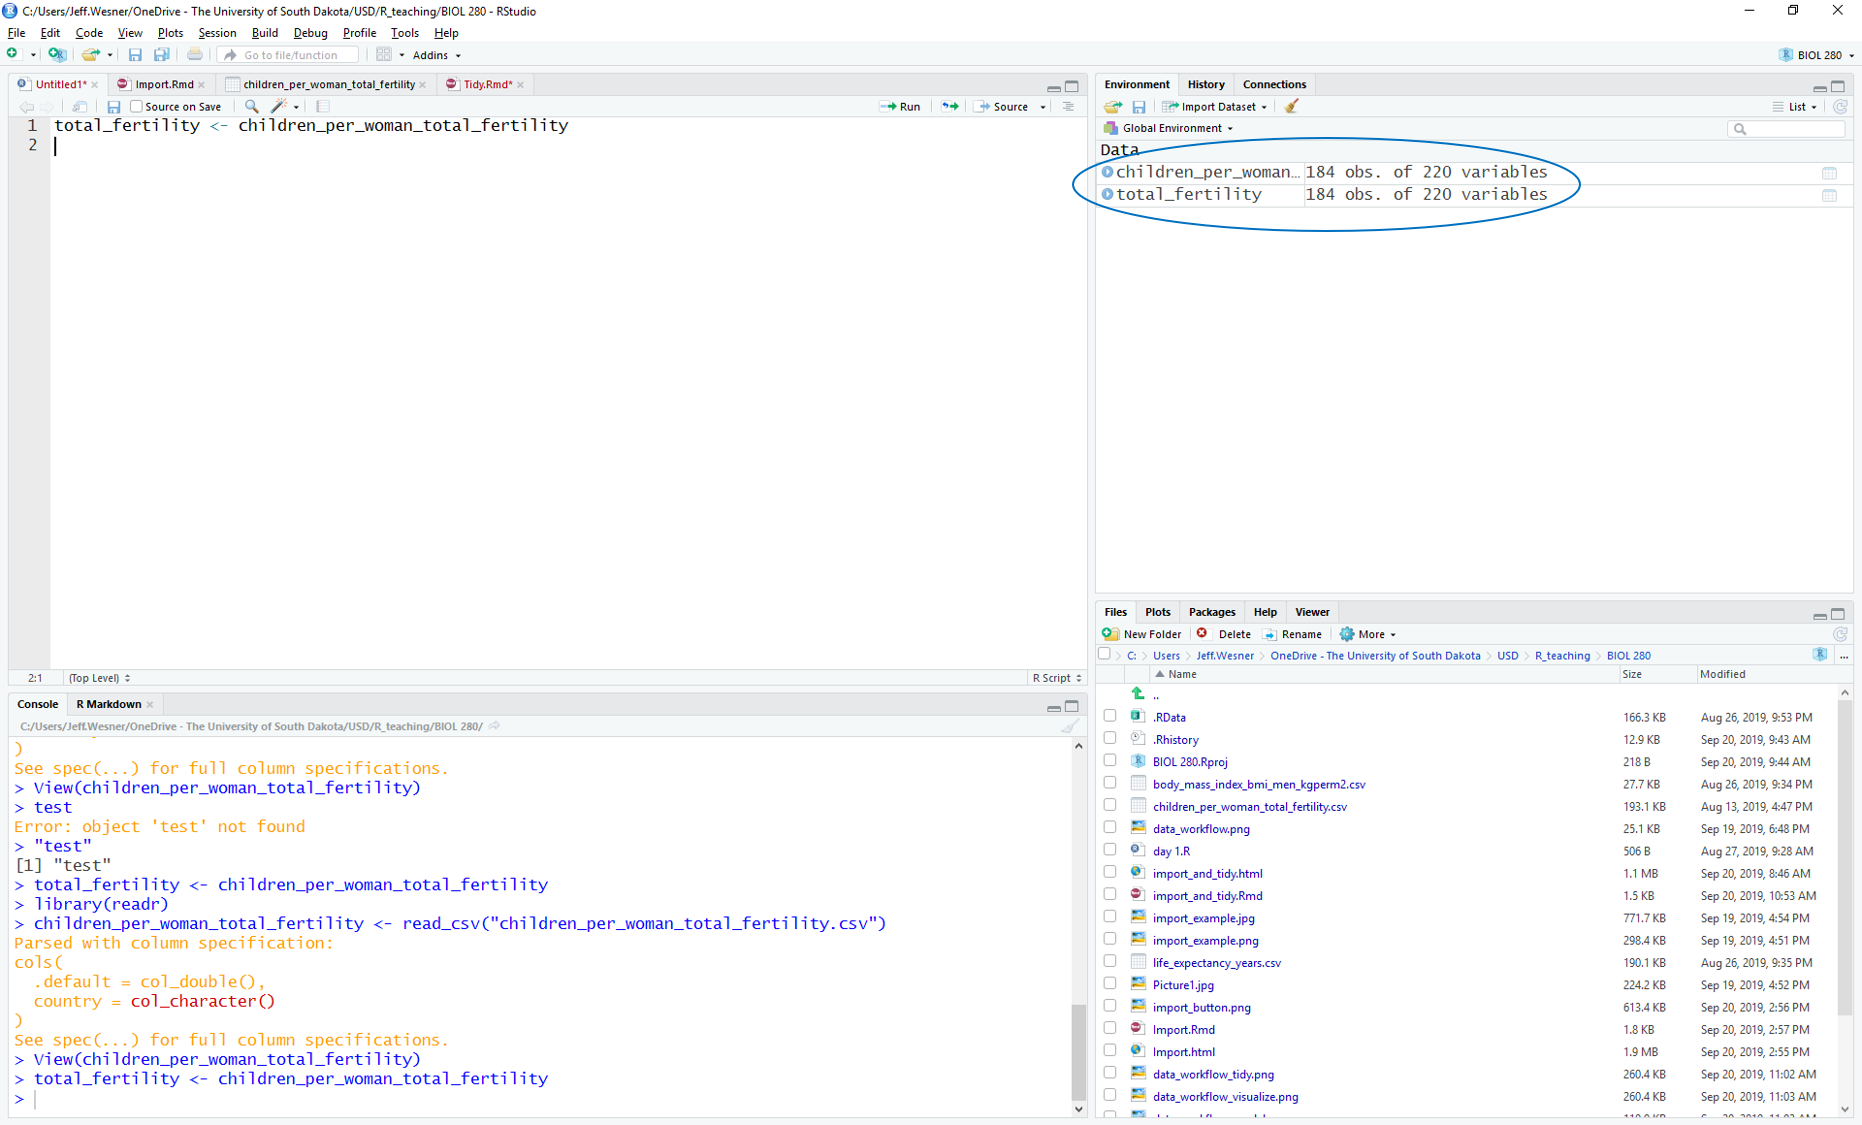
\includegraphics{first_code.png}

\subsubsection{Install some packages}\label{install-some-packages}

``Packages'' are simply shortcuts for coding that other people have
developed and released to the world. R has a
\href{https://cran.r-project.org/web/packages/available_packages_by_name.html\%20of\%20external\%20packages}{huge
library of external pakckages}. We're going to use two of them -
\emph{tidyverse} and \emph{janitor}. Getting these packages involves two
steps:

\begin{enumerate}
\def\labelenumi{\arabic{enumi})}
\tightlist
\item
  Install the packages to your computer. You only have to do this once.
  Paste the code below in your script and run it.
\end{enumerate}

\begin{Shaded}
\begin{Highlighting}[]
\KeywordTok{install.packages}\NormalTok{(}\StringTok{"tidyverse"}\NormalTok{)}
\KeywordTok{install.packages}\NormalTok{(}\StringTok{"janitor"}\NormalTok{)}
\end{Highlighting}
\end{Shaded}

\begin{enumerate}
\def\labelenumi{\arabic{enumi})}
\setcounter{enumi}{1}
\tightlist
\item
  Tell R that you want to use the package in this session by typing
  \emph{library(INSERT PACKAGE NAME)} (replace with the actual package
  name). Try typing the code below and clicking Run.
\end{enumerate}

\begin{Shaded}
\begin{Highlighting}[]
\KeywordTok{library}\NormalTok{(tidyverse)}
\end{Highlighting}
\end{Shaded}

\begin{verbatim}
## -- Attaching packages ----------------------------------------------------------------- tidyverse 1.2.1 --
\end{verbatim}

\begin{verbatim}
## v ggplot2 3.2.0          v purrr   0.3.2     
## v tibble  2.1.3          v dplyr   0.8.3     
## v tidyr   0.8.3.9000     v stringr 1.4.0     
## v readr   1.3.1          v forcats 0.4.0
\end{verbatim}

\begin{verbatim}
## -- Conflicts -------------------------------------------------------------------- tidyverse_conflicts() --
## x dplyr::filter() masks stats::filter()
## x dplyr::lag()    masks stats::lag()
\end{verbatim}

\begin{Shaded}
\begin{Highlighting}[]
\KeywordTok{library}\NormalTok{(janitor)}
\end{Highlighting}
\end{Shaded}

\begin{verbatim}
## 
## Attaching package: 'janitor'
\end{verbatim}

\begin{verbatim}
## The following objects are masked from 'package:stats':
## 
##     chisq.test, fisher.test
\end{verbatim}

\subsubsection{Tidy the data}\label{tidy-the-data-1}

Your dataset has a column for country and a bunch of other columns for
years. The numbers represent the number of children born per woman for a
given combination of country and year. You can do a lot with this. For
example, the code below will calculate the mean, median, and standard
deviation of fertility in the year 1801. The dollar sign just indicates
that you want to perform an operation on a certain column within a
dataset:

\begin{Shaded}
\begin{Highlighting}[]
\KeywordTok{mean}\NormalTok{(total_fertility}\OperatorTok{$}\StringTok{'1801'}\NormalTok{) }\CommentTok{#find the column called 1801 in the dataset called "total_fertility" and caculate the mean}
\KeywordTok{median}\NormalTok{(total_fertility}\OperatorTok{$}\StringTok{'1801'}\NormalTok{) }\CommentTok{#find the column called 1801 in the dataset called "total_fertility" and caculate the mean)}
\KeywordTok{sd}\NormalTok{(total_fertility}\OperatorTok{$}\StringTok{'1801'}\NormalTok{) }\CommentTok{#find the column called 1801 in the dataset called "total_fertility" and caculate the mean}
\end{Highlighting}
\end{Shaded}

You can also plot the data like this:

\begin{Shaded}
\begin{Highlighting}[]
\KeywordTok{plot}\NormalTok{(total_fertility}\OperatorTok{$}\StringTok{'1801'}\NormalTok{)}
\end{Highlighting}
\end{Shaded}

How would you interpret this plot?

The functions above are extremely useful for quick checks of your data.
But they quickly become tedious with larger datasets. For example, you
have 200 years worth of fertility data. We need a better way to organize
it and automate some processes. You don't want to compute a mean 200
times by hand!

The code below will make the dataset ``long'' instead of ``wide'' so
that we have only three columns (country, year, children\_per\_woman),
instead of 184 columns.

\begin{Shaded}
\begin{Highlighting}[]
\NormalTok{total_fertility_long <-}\StringTok{ }\NormalTok{total_fertility }\OperatorTok\StringTok{ }
\StringTok{  }\KeywordTok{gather}\NormalTok{(}\DataTypeTok{key =}\NormalTok{ year, }\DataTypeTok{value =} \StringTok{"children_per_woman"}\NormalTok{, }\OperatorTok{-}\NormalTok{country)}
\end{Highlighting}
\end{Shaded}

In words, this says ``create a new file called total\_fertility\_long.
In that file take the data from total\_fertility \emph{and then} gather
all the columns and stack them, but ignore the country column in this
operation''. More generally, this procedure does this:

\begin{figure}
\centering
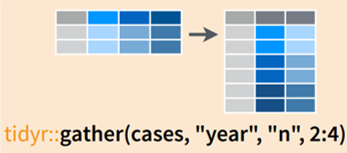
\includegraphics{gather.png}
\caption{}
\end{figure}

\emph{gather()} is one function that the \emph{tidyverse} packages does.
\emph{Tidyverse} provides a lot of useful shortcuts for arranging your
data. For example, you could also filter the dataset so that it only
contains data from 1800, 1900, and 2000:

\begin{Shaded}
\begin{Highlighting}[]
\NormalTok{total_fertility }\OperatorTok\StringTok{ }
\StringTok{  }\KeywordTok{gather}\NormalTok{(}\DataTypeTok{key =}\NormalTok{ year, }\DataTypeTok{value =} \StringTok{"children_per_woman"}\NormalTok{, }\OperatorTok{-}\NormalTok{country) }\OperatorTok\StringTok{ }
\StringTok{  }\KeywordTok{filter}\NormalTok{(year }\OperatorTok{==}\StringTok{ }\DecValTok{1800}\OperatorTok{|}\NormalTok{year }\OperatorTok{==}\StringTok{ }\DecValTok{1900}\OperatorTok{|}\StringTok{ }\NormalTok{year }\OperatorTok{==}\StringTok{ }\DecValTok{2000}\NormalTok{)}
\end{Highlighting}
\end{Shaded}

We will primarily use just two functions - \emph{gather()} and
\emph{filter()}. But there are lots of extras to explore if you're
interested here -
\url{https://www.rstudio.com/wp-content/uploads/2015/02/data-wrangling-cheatsheet.pdf}


\end{document}
